\documentclass[10pt, letterpaper]{article}

\usepackage{mathtools}
\usepackage{amsmath,amssymb,amsfonts,amsthm}
\usepackage{mathabx}
\usepackage{mathrsfs}
\usepackage[onehalfspacing]{setspace}
\usepackage{hyperref}
\usepackage{libertine}
\usepackage{fontspec}
\usepackage{semantic}
\usepackage{multicol}
\usepackage[dvipsnames]{xcolor}
\usepackage[numbers]{natbib}
\usepackage{pifont}
\usepackage{tabularx}
\usepackage{booktabs}
\usepackage{xspace}
\usepackage{circledsteps}
\usepackage{listings}
\usepackage{lstautogobble}
\usepackage{tikz, tikz-qtree, tikz-qtree-compat}
\usepackage[justification=centering]{caption}

\usetikzlibrary{shapes,arrows}
\usetikzlibrary{decorations.markings}
\newcommand\tikzmark[2]{\tikz[overlay,remember picture, anchor=base] \node (#1) {#2};}

\newcommand{\key}[1]{\ensuremath{\mathtt{#1}}}
\newcommand{\Surface}{\ensuremath{\lambda_{\mathtt{IFC}}^\star}\xspace}
\newcommand{\SurfaceOld}{\ensuremath{\lambda_{\mathtt{SEC}}^\star}\xspace}
\newcommand{\CCOld}{\ensuremath{\lambda_{\mathtt{SEC}}^{\Rightarrow}}\xspace}
\newcommand{\CC}{\ensuremath{\lambda_{\mathtt{IFC}}^{c}}\xspace}
\newcommand{\DynIFC}{\ensuremath{\lambda_{\mathtt{SEC}}}\xspace}
\newcommand{\GSLRef}{\ensuremath{\mathrm{GSL}_\mathsf{Ref}}\xspace}
\newcommand{\unk}{\key{\star}\xspace}

\setmonofont[Scale=0.9]{Iosevka}

\lstdefinestyle{tt}{
  basicstyle=\ttfamily\small,
  autogobble,
  escapechar=|
}

\colorlet{green}{PineGreen}
\colorlet{red}{RedOrange}

\title{PhD Dissertation Proposal: \\
  The Holy Grail of Gradual Security}

\author{Tianyu Chen \\ Computer Science, Indiana University}
\date{March 2024}

\begin{document}

\maketitle

\fbox{
	\parbox{0.9\linewidth}{ \textbf{My thesis:} \\ It \textit{is possible} to
    design a gradual security-typed programming language that satisfies both
    noninterference and the gradual guarantee, by excluding the unknown label
    \unk from runtime security labels. } }
\vspace{10pt}

\section{Programming Languages Can Enforce Security}

With the development of digital society, people are increasingly concerned about
the confidentiality of their personal data and the integrity of their online
assets. Increasingly relying on computing devices and the Internet in their
daily life, people fear that sensitive personal information, such as social
security numbers, medical records, bank account balances... may be revealed to
malicious third parties. People also worry that their digital photo albums,
signatures on online legal documents, spreadsheets in cloud storage... may be
tampered and manipulated by potential attackers.

Indeed, the fears are justified by recent news events. In 2018, the Cambridge
Analytica scandal hit the world headlines, where the data collected from 87
million social media users was misused without their consent
~\citep{cadwalladr2018facebook,kitchgaessner2017cambridge,gonzalez2019global,hinds2020wouldn}.
In the healthcare sector, from 2005 to 2019, 249 million people were
affected by data breaches that caused exposure of sensitive medical
data~\citep{seh2020healthcare}. Researchers have found ways to tamper with the
analytics APIs~\citep{pfeffer2018tampering} and damage the integrity of
metadata, such as the numbers of likes, follows, and views, of major social
media platforms~\citep{paquet2017can}. To deal with the security and privacy
challenges of the increasingly digitalized world, the European Union introduced
the General Data Protection Regulation (GDPR) to reform and regulate the
collection and processing of personal data. However, studies show that business
entities experience challenges in complying with GDPR or auditing for
compliance~\citep{smirnova2024understanding}, particularly small-to-medium
size enterprises~\citep{sirur2018we,freitas2018gdpr,harting2021impacts}.

\begin{figure}[tbp]
  \small
  \begin{align*}
    \langle \mathit{RECORD} \rangle ::= & {\color{green} \textbf{\{FirstName=}} \langle \mathit{ID} \rangle {\color{green} \textbf{;}} \\
                               & \enspace {\color{green} \textbf{LastName=}} \langle \mathit{ID} \rangle {\color{green} \textbf{;}} \\
                               & \enspace {\color{green} \textbf{SSN=}} \langle \mathit{SSN} \rangle {\color{green} \textbf{\}}} \\
    \langle \mathit{ID} \rangle     ::= & w , w \in \{ {\color{green} \textbf{A}}, ... {\color{green} \textbf{Z}}, {\color{green} \textbf{a}}, ... {\color{green} \textbf{z}} \}^{+} \\
    \langle \textit{SSN} \rangle    ::= & \langle D \rangle \langle D \rangle \langle D \rangle {\color{green} \textbf{-}}
                                 \langle D \rangle \langle D \rangle {\color{green} \textbf{-}}
                                 \langle D \rangle \langle D \rangle \langle D \rangle \langle D \rangle \\
    \langle D \rangle      ::= & d , d \in \{ {\color{red} \textbf{0}}, ... {\color{red} \textbf{9}} \}
  \end{align*}
  \caption{The user input grammar for a hypothetical application}
  \label{fig:grammar}
\end{figure}

From a technical perspective, ensuring the security and privacy of personal data
typically involves tracking and checking the flow of information. To ensure
confidentiality, data must not flow to inappropriate destinations, so that
sensitive personal information is not revealed; dually, to ensure integrity,
data must not flow from inappropriate sources, so that valuable digital assets
are not corrupted~\cite{sabelfeld2003language,biba1977integrity}. In practice,
such enforcement of the flow of information is often difficult to implement.
Take confidentially for example, software applications accept user input where
selected fields are sensitive, whose confidentiality is required during their
entire life cycle including both parsing and data processing. To rule out
information leaks, neither the sensitive fields, nor any data that depends on
those fields, is allowed to be revealed to a low-privilege observer. Consider a
web application that receives three fields from its user: (1) first name
(2) last name (3) social security number, the grammar of which
is defined in Figure~\ref{fig:grammar}, where terminals are divided into
low-security and high-security. The digits $d$ for social security number, being
confidential to users of the web application, are of high-security, so they are
marked {\color{red} red}, while other terminals, such as the keys of the record
and the strings $w$ for first name / last name, being safe to disclose, are all
of low-security, marked in {\color{green} green}. Consider the following user
input:

\begin{lstlisting}[numbers=none,xleftmargin=0.15\textwidth,style=tt]
{FirstName=Mad;LastName=Hatter;SSN=012-34-5678}
\end{lstlisting}

\noindent It is tedious for the developer of this imaginary web application to track the
security level of data and check for information leaks. Software developers tend
to focus more on functionality in order to meet the tight software release
schedule and budget, thus software security usually only comes as an
afterthought
~\citep{assal2018security,sharma2017aspects,steward2012software}.
Retrofitting security-related code often requires extensive modification to an
existing code-base and it relies on the programmers' skills and experience to
decide when and where such code should be placed. Furthermore, such modification
is error-prone: one single missing check could undermine the security of the
entire application.

\begin{figure*}[tbp]
  \small
  \center
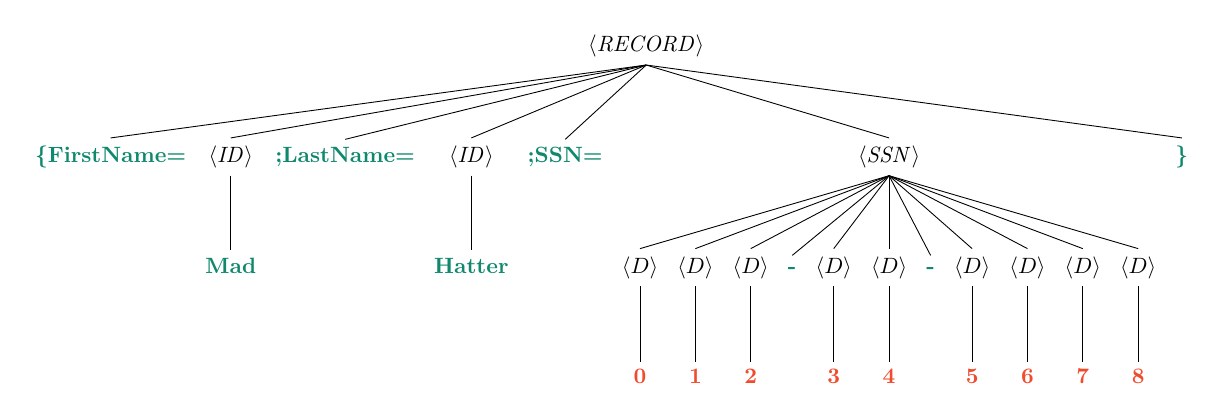
\begin{tikzpicture}[scale=0.8]
\tikzset{level distance=50pt}
\Tree [
  .{ $\langle \mathit{RECORD} \rangle$ }
  {\color{green} \textbf{\{FirstName=}}
  [ .{ $\langle \mathit{ID} \rangle$ } {\color{green} \textbf{Mad}} ]
  {\color{green} \textbf{;LastName=}}
  [ .{ $\langle \mathit{ID} \rangle$ } {\color{green} \textbf{Hatter}} ]
  {\color{green} \textbf{;SSN=}}
                       [ .{ $\langle \mathit{SSN} \rangle$ }
                         [ .{ $\langle D \rangle$ } {\color{red} \textbf{0}} ]
                         [ .{ $\langle D \rangle$ } {\color{red} \textbf{1}} ]
                         [ .{ $\langle D \rangle$ } {\color{red} \textbf{2}} ]
                         {\color{green} \textbf{-}}
                                [ .{ $\langle D \rangle$ } {\color{red} \textbf{3}} ]
                                [ .{ $\langle D \rangle$ } {\color{red} \textbf{4}} ]
                                {\color{green} \textbf{-}}
                                       [ .{ $\langle D \rangle$ } {\color{red} \textbf{5}} ]
                                       [ .{ $\langle D \rangle$ } {\color{red} \textbf{6}} ]
                                       [ .{ $\langle D \rangle$ } {\color{red} \textbf{7}} ]
                                       [ .{ $\langle D \rangle$ } {\color{red} \textbf{8}} ] ]
                       {\color{green} \textbf{\}}}
]
\end{tikzpicture}
\caption{The parse tree generated from the example user input.
  All terminals are represented as labeled values:
  the {\color{red} red} ones, such as the digits of SSN,
  are of high-security, while the {\color{green} green} ones, such as the keys
  of the record and first name / last name, are of low-security.}
\label{fig:parsetree}
\end{figure*}

\clearpage
\bibliographystyle{ACM-Reference-Format}
\bibliography{all.bib}
\bibliography{references.bib}

\end{document}
